\documentclass{standalone}
\usepackage{tikz}

\begin{document}
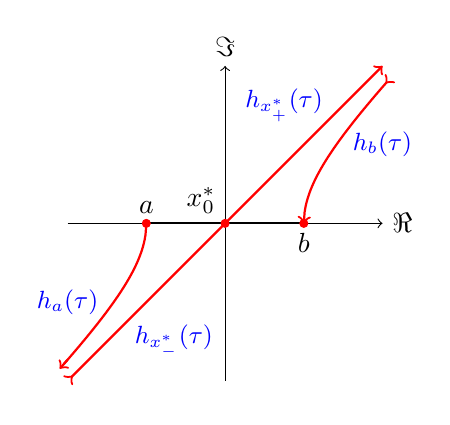
\begin{tikzpicture}
  \draw[->] (-2,0) -- (2,0) node[right] {$\Re$};
  \draw[->] (0,-2) -- (0,2) node[above] {$\Im$};
  \draw[black, thick] (-1,0) -- (1,0);
  \draw[red, thick, <-] (-2.1,-1.84662) -- (-2.0,-1.732);
  \draw[red, thick, domain=-2.05:-1, samples=100] plot (\x,{-sqrt(((\x*\x)-1)});
  \draw[red, thick, >-, domain=-2:0] plot (\x,\x);
  \draw[red, thick, ->, domain=0:2] plot (\x,\x);
  \draw[red, thick, <-<, domain=1:2, samples=100] plot (\x,{sqrt((\x*\x-1)}) -- (2.0,1.732) -- (2.1,1.84662);
  \draw[fill, red] (0,0) circle [radius=.05] node[above left, black] {$x^{*}_{0}$};
  \draw[fill, red] (-1,0) circle [radius=.05] node[above, black] {$a$};
  \draw[fill, red] (1,0) circle [radius=.05] node[below, black] {$b$};
  \draw[fill, blue] (-2,-1) node {\small{$h_{a}(\tau)$}};
  \draw[fill, blue] (-0.65,-1.5) node {\small{$h_{x^{*}_{-}}(\tau)$}};
  \draw[fill, blue] (0.75,1.5) node {\small{$h_{x^{*}_{+}}(\tau)$}};
  \draw[fill, blue] (2,1) node {\small{$h_{b}(\tau)$}};
  \useasboundingbox (-2.2,-2.2) rectangle (2.2,2.2);
\end{tikzpicture}
\end{document}
